\chapter{Intégration de l'énergie dans la conception physique : Cas des vues matérialisées}
\label{chap6}

\epigraph{<< Knowledge is power. >>}{--- \textup{Francis Bacon}}

\NoChapterPrefix \NoChapterNumberInRef {\hypersetup{linkcolor=black} \minitoc}

%% numérotation des figures, des tables et des équations préfixé par le numéro de chapitre
\makeatletter
\renewcommand{\thefigure}{\ifnum \c@section>\z@ \thechapter.\fi
 \@arabic\c@figure}
\@addtoreset{figure}{chapter}
\makeatother

\makeatletter
\renewcommand{\thetable}{\ifnum \c@section>\z@ \thechapter.\fi
 \@arabic\c@table}
\@addtoreset{table}{chapter}
\makeatother

\makeatletter
\renewcommand{\theequation}{\ifnum \c@section>\z@ \thechapter.\fi
 \@arabic\c@equation}
\@addtoreset{equation}{chapter}
\makeatother
%%-----------------------------------------------------------------
%% Résumé
%%-----------------------------------------------------------------


%laisser une page ou deux pages vides, telle est la question !
%\EmptyNewPage
\newpage

%********************************************************************************
%********************************************************************************
\section{Introduction}
Dans l'ère des Big data, la gestion de la consommation d'énergie par les serveurs et centres de données est devenue un enjeu majeur pour les entreprises, les institutions et les pays. Dans les applications centrées sur les données, les systèmes de gestion de base de données sont l'un des principaux consommateurs d'énergie lors de l'exécution des requêtes complexes impliquant de très grandes masse de données. Plusieurs initiatives ont été proposées pour traiter cette problématique, couvrant à la fois les dimensions matérielles et logicielles. Dans ce chapitre, nous nous concentrons sur la conception physique des bases de données, où des structures d'optimisation (par exemple, des index, des vues matérialisées) sont sélectionnées pour satisfaire un ensemble donné de besoins non fonctionnels tels que la performance pour une charge de requêtes. Dans ce chapitre, nous proposons d'abord une initiative, qui intègre la dimension énergétique dans la conception physique lors de la sélection des vues matérialisées, l'une des structures d'optimisation redondantes. Deuxièmement, nous fournissons une formalisation multi-objective du problème de sélection de vue matérialisée, en tenant compte de deux besoins non fonctionnels : la performance et la consommation d'énergie lors de l'exécution d'une charge de requêtes donnée. En troisième lieu, un algorithme évolutionnaire a été développé pour résoudre le problème. Cet algorithme diffère de ceux qui existent déjà en étant interactif, afin que les administrateurs de base de données peuvent ajuster certains paramètres sensibles de l'énergie à l'étape finale d'exécution de l'algorithme en fonction de leurs spécifications. Enfin, des expérimentations intensives sont menées en utilisant notre modèle de coût mathématique et un dispositif réel pour les mesures d'énergie. Les résultats obtenus sont très satisfaisants, ce qui rend l'approche qu'on a développé un moyen très efficace pour économiser l'énergie tout en optimisant les requêtes par le biais de vues matérialisées.

La suite de ce chapitre est organisée comme suit. Dans la première section, nous discutons notre initiative de conception éco-énergétique qui concerne la phase de conception physique du cycle de vie des bases de données. Cette section donne une formulation plus détaillée du problème de sélection de vue sur la base de graphe globale de requêtes, ainsi qu'un exemple de support pour illustrer les relations entre la performance et le comportement de la puissance électrique. Cette section présente également les modèles de coûts utilisés dans notre étude pour estimer les performances et la puissance des requêtes SQL. La section suivante décrit notre méthodologie qui se base sur des algorithmes évolutionnaires pour résoudre notre problème d'optimisation multi-objectifs. L'algorithme et ses paramètres sont expliqués en détail, y compris les étapes de sélection, croisement, mutation et la méthode de pondération. La section suivante présente et discute les résultats expérimentaux basés sur plusieurs scénarios de matérialisation de vues avec différents paramètres et tailles de données. Enfin, la dernière section conclut le chapitre en résumant les principaux résultats.

\section{Pourquoi la conception physique ?}\label{PourquoiConceptionPhysique}
Notre initiative concerne la phase de conception physique. Récemment, plusieurs chercheurs bien connus du milieu universitaire (Stavros Harizopoulos \textit{et al.} \cite{Harizopoulos09}, MIT) et de l'industrie (Goetz Graefe \cite{Graefe08}, HP) ont recommandé de revoir la conception physique en impliquant la dimension d'énergie. Il convient de noter que la configuration physique de la base de données sur le support de stockage est spécifiée dans la phase de conception physique. Plusieurs techniques (structures) d'optimisation telles que les vues matérialisées, les indexes et le partitionnement sont sélectionnées à cette phase pour améliorer les performances d'exécution des requêtes \cite{ElghandourAZZ13}. L'importance de la conception physique a été amplifiée avec l'avance des optimiseurs de requêtes qui sont devenus assez sophistiqués pour faire face aux demandes d'aide à la décision complexes \cite{ChaudhuriN07}. Habituellement, la sélection d'une structure physique est effectuée par le biais des algorithmes utilisant des modèles d'estimation de coûts d'un ou de plusieurs fonctions objectives \cite{Mami12}. Notez que ces modèles de coûts utilisent des paramètres liés à des schémas de base de données, le matériel, la requête, la charge de requêtes et les contraintes (coûts de stockage, les coûts de maintenance, etc.). La \ref{fig:physical-design} illustre le schéma de la conception physique des bases de données. La sélection de ces structures d'optimisation impacte fortement la base de données finale, car elles deviennent une partie de celui-ci. En conséquence, elles peuvent contribuer de manière positive ou négative à l'augmentation de la consommation d'énergie. Par conséquent, l'exploration de la conception physique éco-énergétiques est cruciale pour éviter le gaspillage d'énergie lors de la sélection et le maintien de ces structures d'optimisation. Pour surveiller cette énergie, nous recommandons son intégration dans le processus de conception physique.
 
Dans cette étude, nous proposons une initiative qui intègre l'énergie dans le processus de conception physique en considérant la technique des \textit{vues matérialisées} qui est une structure d'optimisation redondante dont les résultats des requêtes sont stockés et maintenus afin d'optimiser globalement la charge de requêtes \cite{Gupta99}.

\begin{figure}
	\begin{center}
		\includegraphics[scale=0.6]{chapitre6/chap6Fig/physical-design.pdf}
		\caption{Schéma de la conception physique des bases de données.}
		\label{fig:physical-design}
	\end{center}
\end{figure}

Notre initiative visant à réduire la dissipation d'énergie lors de la sélection des structures d'optimisations s'appuie sur la considération de l'énergie comme l'un des objectifs à optimiser. Par conséquent, le processus de sélection de vue matérialisée devient un problème d'optimisation multi-objectifs qui peut impliquer plusieurs objectifs potentiellement contradictoires (par exemple, l'amélioration de performance et d'économie d'énergie). Ce problème dispose d'un ensemble de Pareto \cite{Zhou2011} qui représente l'ensemble des solutions optimales dans les deux objectifs. Les algorithmes évolutionnaires multi-objectifs (AEMOs) sont une approche appropriée pour s'approcher de la \textit{frontière d'efficacité de Pareto} en une seule exécution \cite{Zhou2011}. Les AEMOs ont montré leurs efficacités pour résoudre plusieurs problèmes (par exemple, problème du voyageur de commerce). Comme il est impossible d'avoir une solution unique qui optimise simultanément les deux objectifs, l'utilisation d'un algorithme qui offre aux administrateurs de bases de données (DBA) de nombreuses solutions alternatives situées sur ou près de la frontière d'optimalité de Pareto est d'une grande valeur pratique \cite{Deb02}. A cet effet, nous utilisons l'algorithme élitiste : \textit{Non-Dominated Sorting Genetic Algorithm II} (NSGA-II) \cite{Deb02}. De plus, nous offrons aux DBAs la possibilité de favoriser une fonction objective sur une autre. Pour satisfaire cette exigence, nous avons appliqué la méthode d'agrégation des sommes pondérées qui attribue un poids à chaque fonction objective afin d'avoir une seule solution à déployer par le DBA.

\section{Démarche d'intégration de l'énergie dans le problème de sélection des vues}\label{subsec:ViewSelectionProblem}
Dans cette section, nous présentons en détail notre initiative qui concerne la phase de conception physique du cycle de vie des bases de données. L'initiative vise à proposer des structures d'optimisation qui répondent aux besoins et aux exigences des utilisateurs en termes de performances des requêtes et de l'énergie consommée. La phase de conception physique est comme un entonnoir pour les autres phases du cycle de vie car elle intègre plusieurs paramètres à partir de ces phases. En raison de la diversité des structures d'optimisation, nous considérons le cas des vues matérialisées. Dans la section suivante, nous discutons les différentes possibilités d'intégrer l'énergie dans le processus de sélection de vue.

% \begin{figure}
% 	\centering
% 	\includegraphics[scale=0.5]{chapitre6/chap6Fig/db-design.pdf}
% 	\caption{A systematic view of database design life-cycle.}
% 	\label{fig:db-design}
% \end{figure}

%\section{$\mathcal{PSV}$ avec le scénario d'énergie comme un $\mathcal{BNF}$}
Rappelons que le $\mathcal{PSV}$ consiste à trouver un ensemble approprié de vues pour la matérialisation tout en satisfaisant un ensemble donné de $\mathcal{BNF}$ (comme la performance des requêtes, la fiabilité, l'utilisabilité, etc). Les vues matérialisées sélectionnées doivent répondre à un ensemble de contraintes telles que le coût de stockage, les coûts de maintenance, etc.

Si on veut intégrer l'énergie dans la sélection des vues matérialisées, on doit l'attribuer à l'une des entrées des formalisations suivantes :
\begin{enumerate}
\item \textbf{La base de données comme référentiel pour stocker et gérer l'énergie} : La consommation d'énergie peut être stockée dans une base de données. Projet MIRABEL \cite{Siksnys12} est un exemple de ce scénario.
\item \textbf{L'énergie comme une contrainte} : Ce scénario est possible; par exemple, un DBA veut sélectionner un ensemble de vues matérialisées sous une contrainte d'énergie bien connue. En règle générale, ce n'est facile de l'estimer a priori.
\item \textbf{Énergie en tant que $\mathcal{BNF}$} : Si le DBA est plus sensible à l'énergie, il peut la considérer comme le principal objectif de sa sélection, comme il peut la combiner avec un autre objectif, tel que le coût de traitement des requêtes.
\end{enumerate}

Dans notre étude d'intégration d'énergie, on considère les scénarios 2 et 3.
Pour le reste de notre étude, nous considérons principalement le scénario 3 et nous donnons quelques résultats préliminaires en considérant le scénario 2 dans la partie expérimentale (\ref{subsubsec:ImpactPower} [page \pageref{subsubsec:ImpactPower}]).

\section{$\mathcal{PSV}$ avec le scénario d'énergie comme un $\mathcal{BNF}$}
Dans cette section, nous présentons tous les ingrédients nécessaires pour mener à bien le processus de sélection des vues matérialisées. Ce processus se résume en trois étapes : (i) la formalisation du $\mathcal{PSV}$, (ii) la définition des modèles de coût d'estimation de chaque fonctions objectives et (iii) la méthodologie de sélection.

\subsection{Formalisation du $\mathcal{PSV}$}
Dans notre étude, le $\mathcal{PSV}$ est formalisé comme suit : étant donné (i) un schéma de base de données $DB$; (ii) une charge de requêtes $W$; (iii) une contrainte stockage $S$; (iv) une contrainte de temps de maintenance $T$; (v) deux $\mathcal{BNF}$ représentant la consommation d'énergie et les coûts de traitement des requêtes.
Le $\mathcal{PSV}$ consiste à sélectionner un ensemble de vues matérialisées $MV = \{V_1, V_2, \cdots , V_m\}$, tout en réduisant le coût de traitement des requêtes, et en économisant la consommation d'énergie, de telle sorte qu'on aurait une taille des vues sélectionnées inférieure à $S$ et une durée totale de maintenance inférieure à $T$.
Les contraintes indiquent que le $\mathcal{PSV}$ est étudié suivant des ressources limitées, par exemple, l'espace de stockage et le temps de maintenance.

Comme mentionné précédemment, le $\mathcal{PSV}$ est prouvé être NP-complet, en raison de la grande taille d'espace de recherche des solutions possibles. Dans notre cas, le $\mathcal{PSV}$ devient encore plus complexe, puisque nous considérons deux fonctions objectives (minimisation de l'énergie et du temps). Par conséquent, trouver de bonnes solutions dans un délai acceptable est un défi supplémentaire à ce problème.
Ceci nous motive, dans cette première étude, de traiter les requêtes de type OLAP en lecture seule. Ces derniers consomment une quantité d'énergie majeure dans les entrepôts de données, car elles sont caractérisées par une longue durée d'exécution et une utilisation intense de ressources \cite{Kunjir12}.

\subsection{Modèle de coût}
Notre objectif est de sélectionner des vues matérialisées qui assurent un bon compromis entre deux coûts : les performances des requêtes et la consommation d'énergie. En conséquence, nous avons besoin de modèles mathématiques pour estimer ces coûts. Dans cette section, nous présentons les étapes nécessaires pour créer les modèles de coûts. Dans le \ref{chap4}, nous avons proposé une approche logicielle basée sur une étude empirique pour trouver les paramètres clés ayant un impact sur la performance et l'énergie lors de l'exécution d'une requête, et pour déterminer le niveau approprié afin de construire notre modèle. L'étude empirique sélectionne également l'algorithme mathématique approprié qui décrit le comportement des requêtes SQL en fonction du $\mathcal{BNF}$. Ces choix sont cruciaux parce qu'ils affectent la précision du modèle final.
Dans ce chapitre, nous nous sommes basés sur le modèle proposé dans le \ref{chap4} pour la sélection des vues matérialisées.

%En supposant que le $\mathcal{BNF}$ $ est l'énergie, les principales étapes de l'élaboration de notre modèle de coûts sont (Figure \ ref {fig: costmodel-méthodologie}):

\begin{table}
%\small
%\footnotesize
%\scriptsize
\caption {Les notations des paramètres du modèle de coût.} \label{tab:cost-param}
%\rowcolors{0}{}{lightgray}
\centering
    \begin{tabular}{ll}
    %\hline\noalign{\smallskip}
    \toprule
    \textbf{Paramètre} & \textbf{Définition} \\ \midrule
    %\noalign{\smallskip} \hline \noalign{\smallskip}
    $\alpha_{cpu}$ & le temps d'effectuer une opération d'E/S \\
    $\alpha_{es}$ & le temps d'effectuer une opération CPU \\
    $\alpha_{net}$ & le temps d'effectuer une opération de communication \\
    $\beta_{cpu}$ & la puissance électrique d'effectuer une opération d'E/S \\
    $\beta_{es}$ & la puissance électrique d'effectuer une opération CPU \\
    $\beta_{net}$ & la puissance électrique d'effectuer une opération de communication \\
    %\noalign{\smallskip} \hline \noalign{\smallskip}
    \midrule
	$m$ & taille de la mémoire tampon pour l'opération de tri \\
	$block$ & taille d'une page dans le SGBD \\
	$L$ & bande passante du réseau \\
	$T_i$ & la taille de la table $i$ \\
	$f_q$ & la fréquence d'exécution de la requête $q$ \\
	$f_v$ & la fréquence de mise à jour de la vue $v$ \\
	%\noalign{\smallskip} \hline \noalign{\smallskip}
	\midrule
    $t_i$ & nombre de tuples d'entrée pour l'opérateur $i$ \\
    $p_i$ & nombre de pages d'entrée pour l'opérateur $i$ \\
    $f$ & sélectivité d'index \\
    $s$ & la taille de la relation d'entrée pour l'opérateur de tri \\
    $n_{hash}$ & nombre de clauses de hachage en phase de construction \\
    $p_{hash}$ & nombre de partitions de hachage en phase de sondage \\
    $p_{outer/inner}$ & nombre de pages pour l'opérateur de jointure \\
    $t_{outer/inner}$ & nombre de tuples pour l'opérateur de jointure \\
    $n_{group}$ & nombre de colonnes de groupement \\ \bottomrule
    %\noalign{\smallskip} \hline
    \end{tabular}
\end{table}

Les paramètres d'entrée qui peuvent être pris en compte dans la construction de modèles de coût sont énumérés dans le \ref{tab:cost-param}. Dans la section qui suit, nous allons détailler le développement de nos modèles de coûts.

\subsubsection{Modèle de coût d'énergie}\label{subsec:PowerCostModel}
La consommation d'énergie peut être réduite soit par la réduction de la consommation moyenne d'énergie soit le temps d'exécution des requêtes. Puisque les optimisations visant l'amélioration des performances des requêtes sont largement étudiées, dans ce travail, nous nous concentrons sur la partie puissance de l'\ref{eq:energy} (page \pageref{eq:energy}). La première étape consiste à modéliser la puissance afin d'estimer sa consommation par les requêtes. À cette fin, nous nous sommes basés sur notre modèle de coûts d'énergie proposé dans le \ref{chap4}. Le processus de construction de ce modèle est décrit dans la suite de cette section.

\paragraph{Paramètres du modèle de coût}\label{subsubsec:ModelParameters}
Dans un SGBD traditionnel, le coût d'exécution de la requête est traité comme une combinaison linéaire de trois composantes : le coût de CPU, le coût d'E/S et le coût de communication \cite{Xu13}. Nous suivons la même logique pour proposer un modèle de coût de l'énergie pour une charge de requêtes.
Pour traiter les tuples, chaque opérateur dans une requête doit effectuer des tâches de CPU et/ou d'E/S. Le coût de ces tâches est la puissance électrique active consommée afin de les terminer. Dans cette étude, nous nous concentrons sur une configuration de serveur centralisée. Ainsi, le coût de communication est ignoré.
Plus formellement, pour une charge de requêtes donnée $W$ de $n$ requêtes $\{Q_1, Q_2, \dots, Q_n\}$. Le modèle de coût de l'énergie pour l'ensemble de requêtes est défini comme suit :
\begin{equation}
Puissance(W) =  \frac{\sum_{i=1}^{n} Puissance(Q_i) \times Temps(Q_i)}{Temps(W)}
\end{equation}
$ Temps(Q_i)$ et $Temps(W)$ représentent respectivement, le temps d'exécution de la requête $i$ et de la charge $W$. Nous obtenons ces facteurs à partir de notre modèle de coût de performance que nous allons décrire dans la section suivante.
Comme mentionné précédemment, la $Puissance(Q_i)$ dépend du nombre d'opérations algébriques de la requête $Q_i$. Pour illustrer cela, soit $m_i$ le nombre de ces opérations $\{OP_1, OP_2, \dots, OP_{m_i}\}$. Le coût $Puissance(Q_i)$ d'une requête $i$ est donné par l'équation suivante : % TODO: revoir l'indice m !
\begin{equation} \label{eq:power-cost-model}
Puissance({Q_i}) = \beta_{cpu} \times \sum_{j=1}^{m_i} COUT\_CPU_j + \beta_{es} \times  \sum_{j=1}^{m_i} COUT\_ES_j
\end{equation}
Où $\beta_{cpu}$ et $\beta_{es}$ sont les paramètres du modèle (à savoir, les unités du coût d'énergie) pour les opérateurs.
Le $COUT\_ES$ est le nombre prévu de \textit{E/S} requis pour l'exécution d'un opérateur spécifique.
Le $COUT\_CPU$ est le nombre prévu de \textit{Cycle de CPU} et de \textit{lecture du mémoire cache} que le SGBD doit exécuter pour un opérateur spécifique.
Ces paramètres sont calculés par rapport aux nœuds (opérateurs) actuellement matérialisés.
Un résumé des formules utilisées pour calculer les coûts d'E/S et CPU pour chaque opérateur de base peut être trouvée dans le \ref{tab:op-cost-param} avec une partie des symboles déjà introduits dans le \ref{tab:cost-param}. Ces formules sont simplifiées à partir du modèle de coût utilisé par l'optimiseur de PostgreSQL.

\begin{table}
%\small
%\footnotesize
%\scriptsize
\caption {Les paramètres du modèle de coût pour les opérateurs SQL.} \label{tab:op-cost-param}
\centering
    \begin{tabular}{lll}
    \toprule
    \textbf{Paramètre} & \textbf{Coût d'E/S} & \textbf{Coût de CPU} \\
	\midrule
    Accès séquentiel & $p_{seq} $ & $t_{seq} $ \\
    Accès par index & $p_{index} $ & $t_{index} \cdot f $ \\
    Accès par bitmap & $p_{bitmap} $ & $t_{bitmap} \cdot f $ \\
    Jointure par boucle imbriquée & $p_{outer}+p_{inner}$ & $t_{outer} \cdot t_{inner} $ \\
    Jointure par tri-fusion & $p_{outer}+p_{inner}$ & $t_{sort(outer)}+t_{sort(inner)} $ \\
    Jointure par hachage & $p_{outer}+p_{inner}$ & $t_{outer} \cdot n_{hash}+t_{inner} \cdot p_{hash} $ \\
    Tri & \begin{tabular}[c]{@{}l@{}}$p_{sort} , s < m;$\\ $0, else$\end{tabular} & $t_{sort} \cdot log_2(t_{sort})$ \\
    Agrégation & $0$ & $t_{agg} $ \\
    Groupement & $0$ & $t_{group} \cdot n_{group} $ \\
    \bottomrule
    \end{tabular}
\end{table}

\paragraph{Régression polynomiale}\label{subsubsec:PolynomialRegression}
Maintenant, il reste à estimer les paramètres $\beta_{cpu} $ et $\beta_{es} $ de l'\ref{eq:power-cost-model}.
Notre méthodologie utilise la technique de régression pour calculer ces paramètres de coût d'énergie. Nous avons employé la méthode de régression polynomiale multiple, avec un ordre de \textit{m=4}. Le coût de l'énergie $Puissance(Q_i)$ de la requête $Q_i$ est calculé comme suit :
\begin{equation} \label{eq:poly-reg-equation-mv}
\begin{aligned}
Puissance(Q_i) = \beta_0 + \beta_1 (COUT\_ES) + \beta_2 (COUT\_CPU) + \\
\beta_3 (COUT\_ES^2) + \beta_4 (COUT\_CPU^2) + \\
\beta_5 (COUT\_ES \times COUT\_CPU) + \\
\cdots + \\
\beta_{13} (COUT\_ES^4) + \beta_{14} (COUT\_CPU^4) + \epsilon
\end{aligned}
\end{equation}
Où $COUT\_ES $, $COUT\_CPU$ représentent la somme des coûts d'E/S et CPU des opérateurs de la requête respectivement, ces coûts sont fournis par le module de statistiques du SGBD, et $\epsilon$ est un terme de bruit qui fait référence à l'erreur de mesure. Les paramètres $\beta$ sont des coefficients de régression qui seront estimés durant de la phase d'apprentissage. Ainsi, les modèles de régression sont résolus par l'estimation des paramètres du modèle $\beta$, qui est fait avec la méthode des moindres carrés (voir \ref{chap4}).

\subsubsection{Modèle de coût de performance}\label{subsec:PerformanceCostModel}
De la même manière, nous utilisons les opérateurs algébriques pour estimer le temps d'exécution de la requête. Soit $LV$ l'ensemble des vues candidat disponible à partir des nœuds de $\mathcal{GGR}$, et $MV$ ($MV \in LV$) l'ensemble des vues matérialisées. Chaque vue $v \in LV$ possède une fréquence de mise à jour $f_v$ associée. $f_{Q_i}$ est la fréquence de la requête, Ainsi, le modèle de coût de performance pour la charge de requêtes est défini comme suit :
\begin{equation}
Temps(W) =  \sum_{i=1}^{n} f_{Q_i} \times Temps(Q_i)
\end{equation}
Le coût $Temps({Q_i})$ d'une requête $i$ est calculé par l'équation suivante :
\begin{equation} \label{eq:time-cost-model}
Temps({Q_i}) = \alpha_{cpu} \times \sum_{j=1}^{m_i} COUT\_CPU_j + \alpha_{es} \times  \sum_{j=1}^{m_i} COUT\_ES_j
\end{equation}

Où $COUT\_ES$, $COUT\_CPU$ sont déjà décrits. Les paramètres $\alpha$ sont des coefficients spécifiés à notre machine de test, utilisés pour convertir les coûts de requête à des valeurs de temps. $\alpha_{cpu}$ est le temps \textit{CPU} requis pour exécuter un \textit{Cycle de CPU} et $\alpha_{es}$ est le temps \textit{d'E/S} du périphérique pour exécuter une opération d'E/S.

En raison des changements qui peuvent survenir dans les relations de base, les vues matérialisées doivent être tenues à jour. Par conséquent, le coût de maintenance de la vue doit être considéré lors du $\mathcal{PSV}$.
%Le coût de maintenance de vue peut être calculé en utilisant des stratégies telles que la stratégie de maintenance incrémentale ou la stratégie de recalcul.
Dans notre travail, nous supposons une stratégie de maintenance incrémentale, lorsque les relations de base changent, nous calculons les changements produits dans les vues, puis nous étendons ces changements à d'autres vues matérialisées. Le coût de la mise à jour de $MV$ est calculé comme suit :
\begin{equation}\label{eq:maint-cost-model}
 U(MV) = \sum_{v \in MV} f_v \times Co\hat{u}t(v)
\end{equation}
Où $Co\hat{u}t(v)$ est le coût de maintenance de la vue $v$. Il est calculé en additionnant le nombre de changements dans les relations de base à partir de laquelle $v$ est mis à jour. Pour calculer ce changement, nous exploitons les techniques décrites dans \cite{Mistry01}. Dans notre étude, nous considérons le cas du $\mathcal{PSV}$ statique, dans laquelle la charge de requêtes est statique, le cas où la charge de requêtes change, également appelé $\mathcal{PSV}$ dynamique, n'est pas traité dans cette thèse. Cependant, il est important de noter que nos algorithmes peuvent être facilement adaptés en utilisant, par exemple, le modèle de coût proposé dans \cite{Lawrence06b} pour capturer ce changement.

\subsection{Méthodologie de sélection des vues matérialisées}
Dans cette section, nous décrivons notre méthode pour résoudre le $\mathcal{PSV}$. Comme dans les études d'état de l'art, le processus de sélection des vues matérialisées commence principalement par la construction du graphe global de requêtes ($\mathcal{\acrshort[hyper=false]{GGR}}$) qui fusionne tous les plans d'exécution des requêtes de la charge (appelé \textit{Multi-Views Processing Plan} dans \cite{Yang97}). Le $\mathcal{GGR}$ est un graphe acyclique orienté. Il comporte quatre niveaux : le premier niveau contient les nœuds de feuille qui représentent les tables de la base de données. Au deuxième niveau, on trouve les nœuds qui représentent les résultats des opérations algébriques unaires telles que la sélection et la projection. Le troisième niveau contient des nœuds représentant des opérations binaires telles que la jointure, l'union, etc. Le dernier niveau représente les résultats de chaque requête. Chaque nœud intermédiaire du graphe est étiqueté avec son coût d'énergie et de traitement. Un exemple d'un $\mathcal{GGR}$ est représenté sur la \ref{fig:mvpp-component}.

Notant que chaque nœud intermédiaire du $\mathcal{GGR}$ est un candidat pour la matérialisation.
Pour choisir le meilleur $\mathcal{GGR}$ qui a le coût minimum, Yang \textit{et al.} ont proposé deux algorithmes dans \cite{Yang97}. Le premier algorithme génère tous les $\mathcal{GGR}$ possibles et le plan qui a le coût minimum sera choisi. Le second algorithme est basé sur l'optimisation linéaire en nombres entiers, il génère les vues matérialisées candidates qui ont des gains positifs entre le traitement des requêtes et la maintenance des vues, seuls les nœuds candidats avec des gains positifs sont sélectionnés pour être matérialisées. La principale limitation du travail de Yang \textit{et al.} est la scalabilité de l'algorithme utilisé pour construire le $\mathcal{GGR}$, car la génération de tous les plans globaux possibles est impossible pour les applications qui contiennent un grand nombre de requêtes.

Pour faire face à ce problème, Boukorca \textit{et al.} \cite{Boukorca15} ont proposé une nouvelle approche basée sur la structure de données de graphe inspiré du domaine de la conception assistée par ordinateur pour l'électronique (Electronic Design Automation). Le processus de génération est composé de cinq étapes : (1) l'analyse syntaxique de la requête SQL pour identifier les opérations logiques (nœuds), (2) la modélisation des nœuds de jointure par un hypergraphe, où les sommets représentent l'ensemble des nœuds de jointure et l'ensemble des hyper-arêtes représentent la charge de requêtes, (3) le calcul des composants connectés en utilisant les algorithmes de partition des hypergraphes du domaine de conception des circuits électroniques, résultant en un ensemble de composants disjoints de requêtes, chaque composant est représenté par un sous-hypergraphe, (4) la transformation de chaque sous-hypergraphe en un graphe orienté en utilisant un modèle de coût et un ensemble d'algorithmes, (5) la fusion des graphes produits pour générer le graphe global de requêtes ($\mathcal{GGR}$). Pour illustrer ces points, considérons un exemple en utilisant les algorithmes de Boukorca \textit {et al.} \cite{Boukorca15}.

\begin{example}\label{subsec:MotivatingExample}
	\begin{figure}
	\centering
	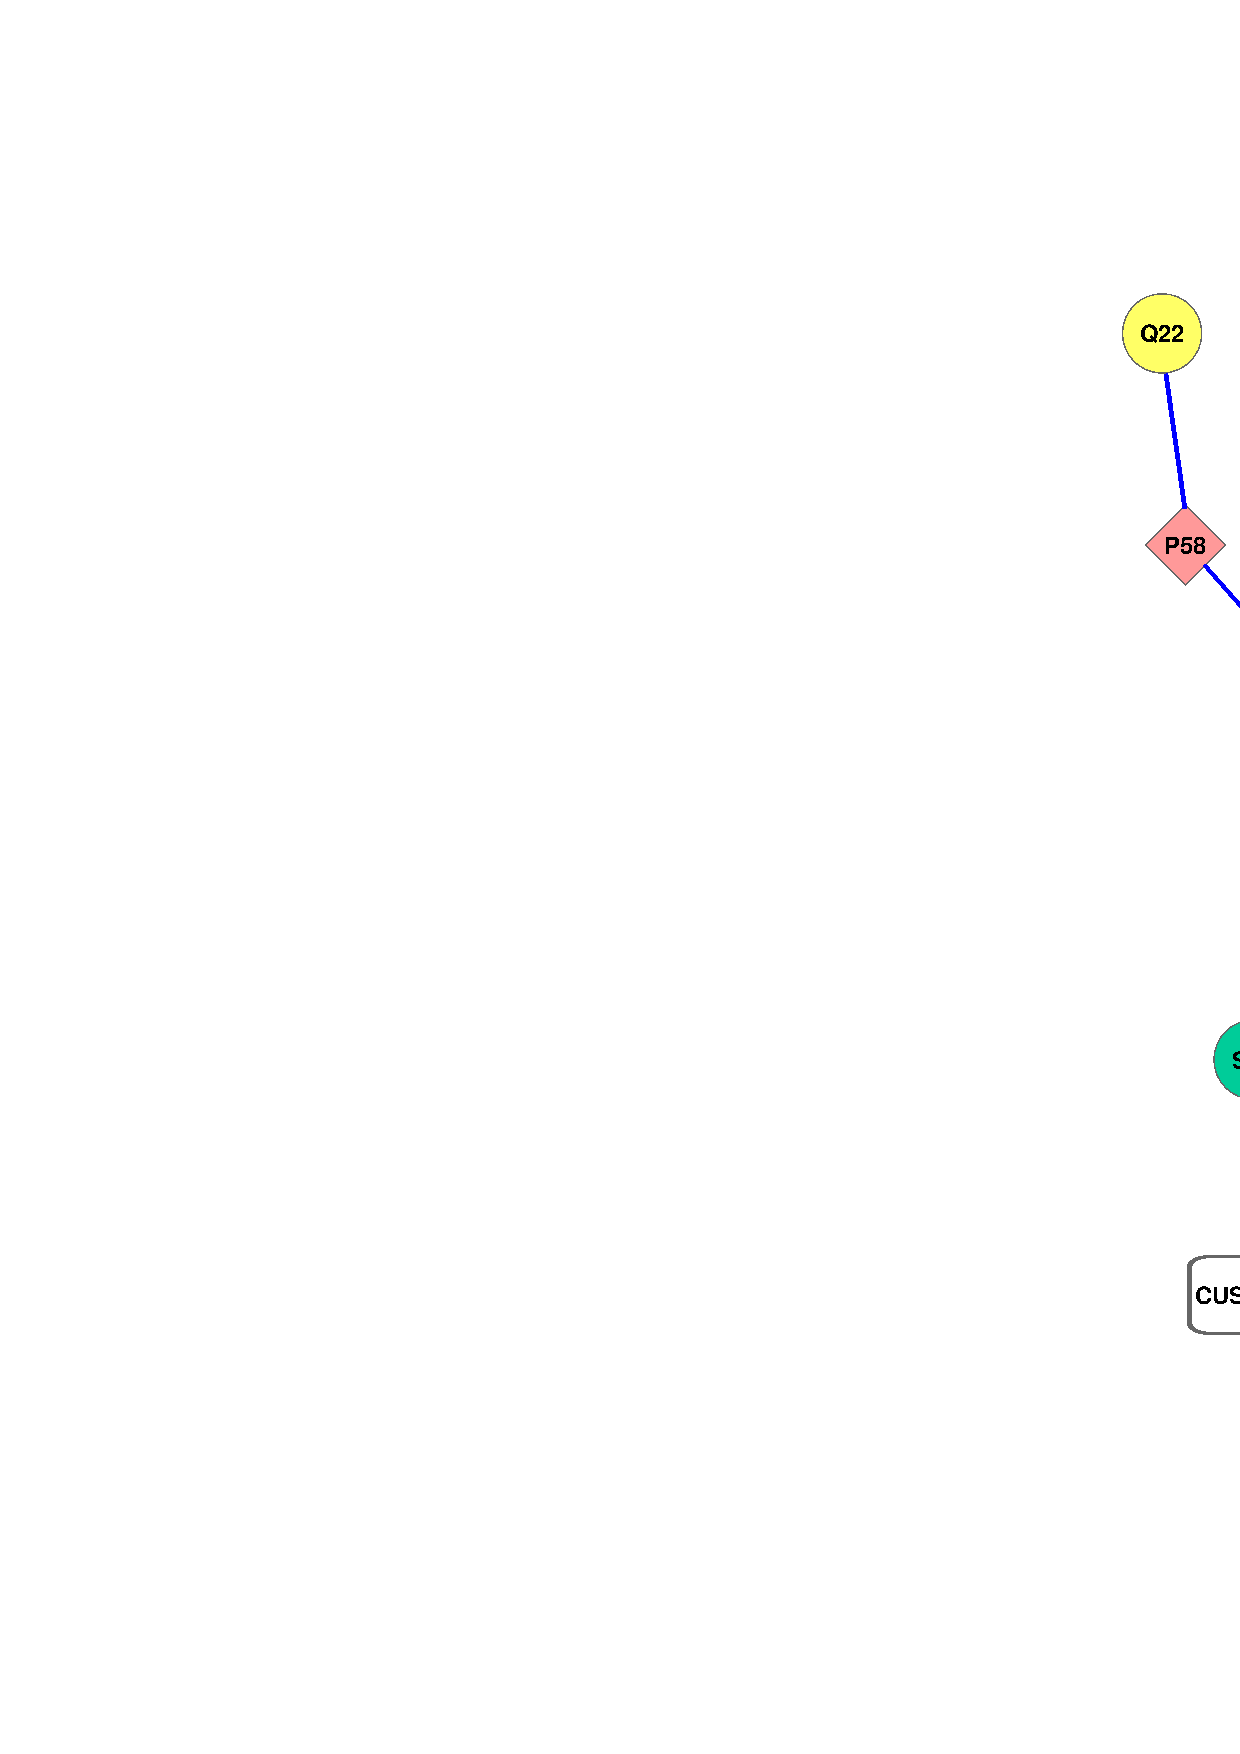
\includegraphics[scale=0.46]{chapitre6/chap6Fig/component.pdf}
	\caption{Exemple d'un $\mathcal{GGR}$ de 7 requêtes.}
	\label{fig:mvpp-component}
\end{figure}

Supposant une charge composée de 7 requêtes de type OLAP générées à partir du \textit{Star Schema Benchmark} (SSB) \cite{Neil09}. Le benchmark contient une table de fait \texttt{Lineorder} (notée $\mathcal{L}$), et quatre tables de dimension : \texttt{Customer} ( $\mathcal{C}$), \texttt{Supplier} ($\mathcal{S}$), \texttt{Part} ($\mathcal{P}$) et \texttt{Dates} ($\mathcal{D}$). Le $\mathcal{GGR}$ correspondant à ces 7 requêtes est représenté dans la \ref{fig:mvpp-component}. À partir de ce plan de requête global, deux alternatives principales sont possibles pour choisir des vues matérialisées pertinentes : (i) matérialiser tous les nœuds ou (ii) matérialiser certains nœuds intermédiaires. Dans cet exemple, nous considérons les nœuds de jointure désignés par $J_i$ comme des vues candidates, le nombre total de configurations possibles est de $2^n$, où $n$ est le nombre de nœuds de jointure ($n = 4$). Le fait que nous avons seulement 16 configurations, nous utilisons une évaluation exhaustive. Pour chaque configuration, nous mesurons le temps d'exécution de la charge de requêtes totale et la consommation de puissance active moyenne. Les ensembles de données, la configuration du système, ainsi que les outils de mesure utilisés dans nos expérimentations seront regroupés dans la \ref{subsec:ExperimentSetup} (page \pageref{subsec:ExperimentSetup}). Les résultats obtenus sont résumés dans le \ref{tab:mvpp-example}. Notant que la configuration peut contenir une ou plusieurs vues matérialisées, aussi, les contraintes de stockage et de maintenance sont relaxées pour des raisons de simplicité.

\begin{table}
\centering
\caption{Les performances et la puissance active de la charge de requêtes pour différentes configurations de vues.} \label{tab:mvpp-example}
    \begin{tabular}{ccc}
    \toprule
    \textbf{Vues matérialisées} & \textbf{Temps (min)} & \textbf{Puissance (watts)} \\
    \midrule
    {$\mathcal{C}$, $\mathcal{P}$, $\mathcal{D}$, $\mathcal{S}$, $\mathcal{L}$} & 10,83 & 16,07 \\
    $J_{32}$ & 3,2 & 19,73 \\
    $J_{31}$ & 5,13 & 18,06 \\
    $J_{31},  J_{32},  J_{30}$ & 2,28 & 21,17 \\
    $J_{29}$ & 6,18 & 17,66 \\
    $J_{29}, J_{31}, J_{30}$ & 2,45 & 21,01 \\
    $J_{29}, J_{30}, J_{31}, J_{32}$ & 1,9 & 23,11 \\
    \bottomrule
    \end{tabular}
\end{table}

Plusieurs notes peuvent être tirées de cette expérimentations :
\begin{itemize}
\item le scénario qui consiste à matérialiser toutes les vues candidates donne la meilleure performance de requête avec la consommation d'énergie la plus élevée. Ainsi, le traitement des requêtes aussi rapide que possible n'est pas toujours la façon la plus économe en énergie, ce qui a déjà été mentionné dans les recherches précédentes, telles que dans \cite{Lang11, Xu10b, Kunjir12};
\item le scénario dans lequel aucune vue n'est sélectionnée offre la pire performance et la plus faible consommation d'énergie. Dans la pratique, cette situation n'est pas favorable puisque l'amélioration de la performance est primordiale pour toute base de données;
\item enfin, matérialisant un certain nombre de vues parmi les candidats est le meilleur compromis. Par exemple, matérialisant $J_{32}$ donne un bon scénario assurant le compromis. Cet exemple nous motive à définir tout d'abord un algorithme de sélection des configurations pertinentes qui permettent d'éviter la recherche exhaustive, puis en choisissant la meilleure solution répondant aux exigences des DBA.
\end{itemize}
\end{example}

\section{Optimisation multi-objectifs}\label{sec:Multi-objective}
Dans les problèmes d'optimisation multi-objectifs, il est essentiel de faire des compromis entre les objectifs.
% Une optimisation multi-objectif générale comprend un ensemble de $n$ paramètres (variables de décision), un ensemble de $k$ fonctions objectifs correspondant à $\mathcal{BNF}$, et un ensemble de $m$ contraintes. L'objectif d'optimisation est de \cite{Zhou2011}:
% \begin{align*}
%   \text{minimiser} \; y &= \; f(x) = (f_1(x), f_2(x), \cdots, f_k (x)) \\
%   \text{avec} \;  e(x) &= (e_1(x), e_2(x), \cdots, e_m(x)) \leq 0 \\
%   \text{et} \;  x &= (x_1, x_2, \cdots , x_n ) \in X \\
%       y &= (y_1, y_2, \cdots , y_k ) \in Y
% \end{align*}
% 
% Où $x$ est le vecteur de décision, $y$ est le vecteur objectif, $X$ est désigné comme l'espace de décision, et $Y$ est appelé l'espace objectif.
Les fonctions objectives de notre problème sont l'énergie (\ref{eq:power-cost-model} [page \pageref{eq:power-cost-model}]) et la performance (\ref{eq:time-cost-model} [page \pageref{eq:time-cost-model}]) respectivement, sous la contrainte de la taille de stockage pour garantir que l'espace total de vues matérialisées est au plus égale à la capacité de l'espace de stockage ($S$), et la contrainte des coûts de maintenance pour garantir que les coûts de mise à jour des vues à matérialiser est inférieure à la durée de maintenance disponible ($U$). Plus formellement, le $\mathcal{PSV}$ multi-objectif pour une solution $MV$ peut être exprimé comme suit :
\begin{align*}
  \text{minimiser} \; f(x) &= (Temps(MV_x), Puissance(MV_x)) \\
  \text{avec} \; e(x) &= S(MV_x) \leq S,\; U(MV_x) \leq U
\end{align*}
Où $S(MV) $ et $U(MV)$ représentent respectivement les coûts de stockage et de maintenance de $MV$.

Rappelons que dans l'optimisation multi-objectifs, il n'existe typiquement pas de solution qui minimise toutes les fonctions objectives simultanément. Par conséquent, des solutions qui ne peuvent pas être améliorées dans l'un des objectifs sans dégrader au moins l'un des autres objectifs sont appelés \textit{des solutions d'optimalité Pareto}. Plus formellement, une solution $x_1$ est dit \textit {domine} une autre solution $x_2$ si $f_i(x_1)\leq f_i(x_2)$ pour tous les indices $i \in \left\{ {1,2,\dots,k } \right\}$ et $f_j(x_1) < f_j(x_2)$ pour au moins une fonction objective $j$.
Une solution $x_1$ est appelé optimale Pareto s'il n'existe pas une autre solution qui la domine. L'ensemble des résultats optimaux de Pareto est appelé la \textit{frontière de Pareto}.
Si l'on considère notre exemple précédent, les valeurs de performance/puissance de toutes les configurations de vues possibles sont tracées dans la \ref{fig:motiv-example}.
\begin{figure}
 \centering
 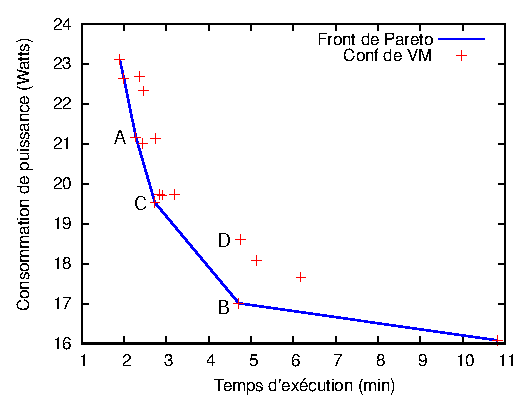
\includegraphics[scale=1.0]{chapitre6/chap6Fig/motiv-example.eps}
 \caption{Exemple de frontière de Pareto lors de la minimisation de deux objectifs (performance et énergie).}
 \label{fig:motiv-example}
\end{figure}
Le point $D$ n'est pas sur la frontière de Pareto car il est dominé par les deux points $A$, $B$, et le point $C$. Les points $A$, $B$ et $C$ ne sont pas strictement dominées par les autres, et donc se trouvent sur la frontière.
Le but ultime est d'identifier des solutions dans l'ensemble d'optimalité de Pareto. Cependant, l'identification de la totalité de cette ensemble, pour notre problème, est pratiquement impossible en raison de sa NP-complétude. Par conséquent, une approche efficace est de rechercher un ensemble de solutions qui représentent l'ensemble d'optimalité de Pareto aussi bien que possible.

\subsection{Techniques de résolutions}\label{subsec:ResolutionsTechniques}
Comme nous l'avons indiqué dans la section ci-dessus, l'optimisation multi-objectifs renvoie un ensemble de solutions Pareto. Cependant, la sélection d'une solution unique pour être déployer dans le système par l'administrateur de base de données peut être très difficile à cause de la multiplicité des solutions retournées. Par conséquent, le problème du choix d'un bon compromis entre les fonctions objectives a été abordé dans la littérature et résolu à l'aide de trois méthodes : (i) méthodes \textit{a priori} (ii) \textit méthodes {interactives} (iii) et méthodes \textit{a posteriori} \cite{Hwang79}. Ces approches sont intégrées aux étapes de traitement de l'optimisation multi-objectifs comme le montre la \ref{fig:multiobjective-resolutions}. La description de chaque approche est la suivante :

\begin{figure}
 \centering
 \includegraphics[scale=0.6]{chapitre6/chap6Fig/multiobjective-resolutions}
 \caption{Procédé d'application d'optimisation multi-objectifs.}
 \label{fig:multiobjective-resolutions}
\end{figure}

\begin{enumerate}
 \item \textbf{Méthodes a priori}. Dans ces méthodes, le DBA intervient \textit{avant} l'exécution du processus d'optimisation. Le DBA définit le compromis entre les fonctions objectives et effectue une seule étape de recherche pour obtenir la solution désirée. Cette méthode est intéressante car elle nécessite une seule étape de recherche. Cependant, il n'est pas simple pour le DBA pour définir les valeurs de compromis sans une connaissance du problème et sans voir des solutions à l'avance, surtout dans notre cas où nous traitons une nouvelle exigence non-fonctionnelle, qui est l'énergie.
 \item \textbf{Méthodes interactives}. Dans le deuxième type de méthodes, le DBA intervient \textit{pendant} l'exécution du processus d'optimisation. Le DBA est invité à définir les valeurs de compromis afin de réorienter progressivement l'espace de recherche vers une solution préférée. Bien que cette méthode peut parvenir à une bonne solution respectant la préférence de DBA, elle requiert toute l'attention de DBA pour évaluer la qualité de chaque solution pendant l'ensemble du processus d'optimisation, ce qui prend du temps pour un grand espace de recherche. En outre, les connaissances spécifiques au domaine du DBA est nécessaire pour prendre de bonnes décisions.
 \item \textbf{Méthodes a posteriori}. Dans le dernier type de méthodes, le DBA intervient \textit{après} l'exécution du processus d'optimisation. Cette méthode fournit aux DBA un ensemble de solutions et le choix de meilleur compromis est reporté à la fin du processus d'optimisation. L'objectif est de montrer ces solutions aux DBA en lui permettant de juger et sélectionner la solution la plus préférée parmi les différentes solutions proposées. Autrement dit, le processus d'optimisation est entièrement automatisé et ne nécessite aucune attention du DBA ou de connaissances de problème. Toutefois, si l'ensemble de résultats est très grand, le processus peut prendre beaucoup de temps pour terminer.
\end{enumerate}

Dans notre étude, nous avons opté pour une approche \textit{a posteriori} pour donner la possibilité aux DBA de \textit{prioriser ou non} l'énergie sur les performances des requêtes. Comme nous l'avons mentionné dans la section précédente, l'évaluation de toutes les solutions candidates est impossible dans notre cas, même pour un petit nombre de relations, en raison de la NP-Complétude du problème. Motivés par ce fait, nous utilisons des algorithmes évolutionnaires pour générer uniquement l'ensemble d'optimum de Pareto, puis nous appliquons la méthode des sommes pondérées à cet ensemble afin d'offrir aux DBA une solution unique. Dans la section suivante, nous discutons en détail les algorithmes proposés pour résoudre notre problème.

\subsection{Algorithmes évolutionnaires}\label{subsec:EvolutionaryAlgorithms}
Les algorithmes évolutionnaires (AE) sont adaptés à des problèmes d'optimisation multi-objectifs, à travers lesquels de grands espaces de recherche peuvent être manipulés, et multiples compromis alternatifs peuvent être générés en une seule phase d'optimisation \cite{Zhou2011}.
L'idée générale derrière les AE est de simuler le processus évolutif naturel dans lequel les individus les plus forts survivront après plusieurs générations. Les détails de la mise en œuvre de notre approche en utilisant les AE sont fournis dans les sections suivantes.

\subsubsection{Représentation des solutions}\label{subsubsec:SolutionRepresentation}
Pour représenter des solutions d'un $\mathcal{GGR}$, toute les vues candidates sont étiquetées. Les solutions sont représentées comme une chaîne binaire de 1 et de 0 de sorte que si une vue particulière est sélectionnée pour la matérialisation, le bit correspondant dans la chaîne de solution prendra 1, et 0 sinon. Par exemple, dans la \ref{fig:mvpp-component}, la solution $\{1,1,1,0\}$ indique que les nœuds \{\texttt{$J_{29}, J_{30}, J_{31}$}\} sont choisis pour la matérialisation.
Pour chaque solution, les fonctions de coût renvoient le coût d'exécution estimé et la consommation d'énergie de la charge de requêtes, ainsi que la taille et le coût de maintenance des vues. La meilleure solution est celle qui a la plus petite valeur des coûts en respectant les contraintes de taille et de maintenance.

\subsubsection{Fonction de fitness}\label{subsubsec:FitnessFunction}
La fonction de fitness mesure la qualité d'une solution (un ensemble de vues sélectionnées pour matérialiser). Nous utilisons l'approche de classement de Pareto comme une fonction de fitness, basée sur l'algorithme génétique NSGA-II proposé par Deb \textit {et al.} \cite{Deb02}, qui utilise explicitement le concept de Pareto dominance dans l'évaluation de la qualité des solutions, où une probabilité de sélection est affectée à chaque solution. Cet algorithme utilise des techniques pour améliorer la convergence et de garantir la diversité et la diffusion des solutions.
Nous utilisons la sélection du tournoi binaire dans lequel les individus sont choisis au hasard de la même manière qu'un << tournoi >>.
La population est classée selon la règle de dominance, puis chaque solution est attribuée une valeur de fitness en fonction de son rang dans la population. Puisque nous voulons minimiser les fonctions objectives, par conséquent, un rang minimal correspond à une meilleure solution.
La solution infaisable, à savoir, une solution qui viole les contraintes est traitée comme suit : essentiellement, une solution réalisable domine toujours une solution infaisable, et si toutes les solutions sont infaisables, ceux avec des violations minimales de contrainte survivent.

\subsubsection{Croisement}\label{subsubsec:Crossover}
Le croisement encourage les permutations des informations entre les différents individus. Il favorise l'héritage de bons gènes d'une génération à une autre et le regroupement de meilleurs individus.
Le croisement moitié uniforme (Half uniform crossover) est utilisé dans notre algorithme évolutionnaire; dans cette technique, la moitié des bits qui sont différents entre les parents seront échangés. A cet effet, la technique calcule le nombre de bits différents en utilisant la distance de Hamming entre les parents. La moitié de ce nombre est le nombre de bits échangés entre les parents pour former des fils. Par exemple, étant donné deux individus $P_1$ et $P_2$, les résultats du croisement sont $C_1$ et $C_2$ :
\begin{equation*}
\begin{array}{l}
  P_1 = \; \{0,1,0,1,1,1,0,1,0\} \; P_2 = \; \{0,1,1,1,1,0,1,1,0\} \\
  C_1 = \; \{0,1,0,1,1,0,1,1,0\} \; C_2 = \; \{0,1,1,1,1,1,0,1,0\} \\
\end{array}
\end{equation*}
Pour générer $C_1$ et $C_2$, l'algorithme compte le nombre de bits différents entre $P_1$ et $P_2$, qui est égale 4, la moitié de ce nombre (donc 2) seront échangées pour créer les nouveaux individus (les bits numéro 6 et 7).

\subsubsection{Mutation}\label{subsubsec:Mutation}
La mutation est la modification aléatoire occasionnelle d'une valeur dans la chaîne de bits. Elle introduit de nouvelles fonctionnalités qui peuvent ne pas être présentes dans aucun membre de la population. La mutation est effectuée en utilisant la méthode de << Bit flip >> dans notre travail. Chaque bit est basculé (commuté d'un 0 à 1 ou vice-versa) en utilisant une probabilité spécifiée. Par exemple, supposons que le $7^{ème}$ bits de l'individu $L_1$ est choisi pour la mutation, la valeur de la chaîne de bits est 1, il sera retourné à 0 avec le taux de mutation spécifiée, la nouvelle personne est $L_1'$ :
\begin{equation*}
\begin{array}{l}
  L_1 = \; \{0,1,0,1,1,0,1,1,0\} \\
  L_1' = \; \{0,1,0,1,1,0,0,1,0\} \\
\end{array}
\end{equation*}

\subsection{Prise de décision}\label{subsec:WeightSum}
Notons que les algorithmes évolutionnaires multi-objectifs produisent un ensemble de solutions. Pour donner aux DBA la possibilité de choisir la meilleure solution parmi cet ensemble selon un compromis fixe (entre les performances des requêtes et l'énergie consommée), nous proposons d'utiliser la méthode des \textit{sommes pondérées des fonctions objectives} (\acrshort[hyper=false]{SPFO}). Dans cette méthode d'agrégation, nous calculons la somme pondérée des fonctions objectives normalisées pour agréger les objectifs en une fonction objectif unique équivalente pour être optimisée. Cette méthode est définie comme suit \cite{Zhou2011} :
\begin{equation}
\begin{aligned}
\text{minimiser} \: y = f(x) &= \sum_{i=1}^{k}\omega_i \cdot f_i(\overrightarrow{x}) \\
\text{tel que} \: \sum_{i=1}^{k}\omega_i &= 1
\end{aligned}
\end{equation}
Où $\omega_i$ sont les coefficients de pondération représentant l'importance relative des $k$ fonctions objectives du problème. Pour normaliser le vecteur des valeurs de fonctions objectives, nous utilisons la formule suivante :
\begin{equation}
x' = \frac{x-min(x)}{max(x)-min(x)}
\end{equation}
Où $x$ est la valeur d'origine et $x'$ est la valeur normalisée.
La méthode des SPFO est bien adaptée lorsque la frontière de Pareto est convexe, tel est le cas dans notre problème. Un exemple de compromis est le point $C$ dans la \ref{fig:motiv-example} ($\omega_1 = 0.5$, $\omega_2 = 0.5$).

L'\ref{algo:energy-vsp} résume le processus de résolution du $\mathcal{PSV}$. Il identifie un ensemble de vues $(MV)$ qui respecte deux contraintes : la taille de stockage et le temps de maintenance, puis il applique la méthode des SPFO pour obtenir la configuration de vues qui a le plus petit coût de traitement possible de la charge de requêtes.

\begin{algorithm}
\caption{$\mathcal{PSV}$ Orienté Énergie}
\label{algo:energy-vsp}
\begin{algorithmic}[1]
\Require $\mathcal{GGR}$, un graphique global de requête
\Ensure $MV$, l'ensemble de vues sélectionnées pour la matérialisation
%\State $MV \leftarrow \emptyset$;
\State $LV \leftarrow \emptyset$;
\State $IterationActuel \leftarrow 0$;
\State
\While{$IterationActuel < MaxEvaluations$ et $aPlusNoeudCandidats(\mathcal{GGR})$}
	\State $CV \leftarrow GAGetNoeudCandidats(\mathcal{GGR})$;
	\State $Co\hat{u}tTemps \leftarrow GetCo\hat{u}tTemps(CV)$;
	\State $Co\hat{u}tPuissance \leftarrow GetCo\hat{u}tPuissance(CV)$;
	\State $Contrainte_i \leftarrow GetContrainte_i(CV)$;
	\If{$Contrainte_i \leq MaxContrainte_i$}
		\State $LV \leftarrow CV$;
	\EndIf
	\State $IterationActuel \leftarrow IterationActuel + 1$;
\EndWhile

\State
\State $WF \leftarrow \emptyset$;
\ForAll {$v \in LV$}
	\State $WF \leftarrow GetPoidFonctions(GetCo\hat{u}tTemps(v),$ $ GetCo\hat{u}tPuissance(v))$;
\EndFor
\State $MV \leftarrow GetMinimum(WF)$;

\State
\State
\Return $MV$;
\end{algorithmic}
\end{algorithm}

Le processus global de notre méthodologie est décrit dans la \ref{fig:methodo}. Ce processus prend une charge de requêtes en entrée, puis il crée le graphique unifié correspondant à cette charge en utilisant les algorithmes de Boukorca \textit{et al.} \cite{Boukorca15}. Les nœuds intermédiaires de ce graphique sont considérés comme des candidats à la matérialisation. Enfin, l'AE est appliqué jusqu'à ce que le nombre maximum d'itérations est atteint. Comme mentionné précédemment, la solution est un ensemble de points de Pareto qui représente la meilleure configuration de vues sur les deux objectifs (la performance et l'énergie). Pour obtenir une solution unique, le DBA définit les paramètres de compromis souhaités dans la méthode des SPFO. La sortie est une configuration de vues unique.

\begin{figure}
	\centering
	\includegraphics[scale=0.5]{chapitre6/chap6Fig/mv-moea.pdf}
	\caption{Le processus de sélection des vues.}
	\label{fig:methodo}
\end{figure}

\section{Évaluation et résultats}\label{sec:Experiments}
Pour évaluer l'efficacité de notre proposition, nous avons mené plusieurs expérimentations. Dans la section suivante, nous présentons notre machine expérimentale pour calculer l'énergie et le jeu de données utilisé ainsi que le simulateur développé.

\subsection{Architecture des expérimentations}\label{subsec:ExperimentSetup}
Nous nous sommes basés sur une configuration similaire à celle utilisée dans le \ref{chap4}. Nous avons utilisé une station de travail Dell Precision T1500 ayant un processeur Intel Core i5 de 2.27GHz, 4 Go de mémoire DDR3. À noter que des techniques comme tension-fréquence dynamique du processeur (DVFS) ne sont pas appliquées dans nos expérimentations. Nous répétons chaque expérience plusieurs fois pour assurer la fiabilité des valeurs observées.

Notre station de travail est dotée de la dernière version du SGBD Oracle 11gR2 sous Ubuntu Server 14.04 LTS avec le noyau Linux 3.13, afin de minimiser les influences indésirables, nous avons désactivé les tâches de fond inutiles, nous avons également vidé le cache du système et le buffer de Oracle dans chaque exécution d'une requête.

Dans les expérimentations, nous utilisons les jeux de données et les requêtes issus du benchmark SSB et TPC-H, avec une taille (facteur d'échelle) de 10 Go et 100 Go. Les données et les requêtes sont générées à l'aide des outils disponibles dans les benchmarks. Les deux benchmarks illustrent des systèmes décisionnels qui examinent de grands volumes de données et exécutent différents types de requêtes avec un degré de complexité élevé. Le SSB est conçu pour le requêtage ad-hoc, le schéma illustre un modèle produits-commandes-fournisseurs contenant une table de faits et 4 tables de dimensions (cf. \ref{fig:ssb-schema}), avec une charge de 13 requêtes décisionnelles caractérisées par un large volume de données. Les requêtes sont exécutées d'une façon isolée dans les expérimentations.
\begin{figure}
 \centering
 \includegraphics[scale=0.6]{chapitre6/chap6Fig/ssb-schema.pdf}
 \caption{Schéma du benchmark SSB.}
 \label{fig:ssb-schema}
\end{figure}

Nous avons développé un outil de simulation utilisant la plate-forme Java. Ce simulateur implémente les algorithmes de Boukorca \textit{et al.} qui génèrent le $\mathcal{GGR}$. L'outil peut extraire automatiquement les caractéristiques de méta-données de la base de données. De plus, il intègre le Framework MOEA\footnote{http://www.moeaframework.org}, qui est une bibliothèque Java pour les algorithmes évolutionnaires multi-objectifs.
Pour chaque configuration de vue matérialisée produite par le framework MOEA, le simulateur calcule les performances et la consommation d'énergie de la charge de requêtes en utilisant les modèles de coûts. Dans notre expérience, nous considérons trois types de configuration de vues matérialisées par : (1) VM-Puissance qui est la configuration qui donne le coût d'énergie minimale, (2) VM-Temps est la configuration avec un coût minimum de temps, (3) VM-Compromis, en utilisant la méthode des SPFO avec $\omega_1 = 0,5$, $\omega_2 = 0,5$.
Les détails de vues matérialisées candidates pour chaque charge de requêtes utilisée dans les expérimentations sont regroupés dans le \ref{tab:moea-exec-time}. Nous supposons que la fréquence d'exécution des requêtes et la fréquence de mises à jour des vues sont uniformes.

\begin{table}
\centering
\caption {Caractéristiques des configurations de vues matérialisées.} \label{tab:mv-charact}
    \begin{tabular}{ll}
    \toprule
    \textbf{Configuration de VM} & \textbf{Caractéristiques de VM} \\
    \midrule
    VM-Puissance & Consommation de puissance minimale \\
    VM-Temps & Temps d'exécution minimale \\
    VM-Compromis & Compromis entre la puissance et le temps \\
    Origine & Sans vue matérialisée \\ 
    \bottomrule
    \end{tabular}
\end{table}

Les paramètres de configuration de l'algorithme évolutionnaire sont résumés dans le \ref{tab:moea-param}. La taille de sélection du tournoi, du croisement, et les probabilités de mutation utilisés dans nos expérimentations sont les valeurs par défaut du framework MOEA. Le nombre maximum d'itération est fixé à 10,000, ce qui permet d'obtenir de bons résultats.
\begin{table}
\caption {Les paramètres de l'algorithme évolutionnaire.} \label{tab:moea-param}
\centering
    \begin{tabular}{ll}
    \toprule
    \textbf{Paramètre} & \textbf{Valeur} \\
    \midrule
    Type d'encodage & chaîne de bits \\
    Méthode de sélection & tournoi binaire \\ 
    taille de la sélection du tournoi & 2 \\ 
    Type de croisement & Half Uniform \\ 
    Probabilité de croisement & 1,0 \\ 
    Type de mutation & Flip Bit \\ 
    Probabilité de mutation & 0,01 \\ 
    Nombre d'évaluations & 10,000 \\
    \bottomrule
    \end{tabular}
\end{table}

%\subsection{La construction des modèle de coût énergétique}\label{subsec:PowerModelBuilding}

\subsection{Résultats}\label{subsec:Results}
Dans cette section, nous présentons les résultats de nos diverses expérimentations.

\subsubsection{Erreurs d'estimations des modèles de coût}\label{subsubsec:CostModelsError}
Dans ce type d'expérimentations, étant donné le coût de performance et d'énergie prédit par nos modèles de coût pour une charge de requêtes, on le compare avec le temps d'exécution réellement observé et la consommation d'énergie du système.
\begin{figure}
  \centering
  \includegraphics[width=0.6\textwidth]{chapitre6/chap6Fig/power-time-error.eps}
  \caption{Les erreurs d'estimation des performances et de la consommation d'énergie de la charge de requêtes.}\label{fig:power-time-error}
\end{figure}
Pour évaluer notre proposition, nous exécutons 30 requêtes de type OLAP générées aléatoirement du benchmark SSB, avec une taille de base de données de 10 Go utilisant les trois configurations de vues matérialisées. Nous optons pour 30 requêtes au lieu des treize requêtes par défaut du SSB pour garantir un grand $\mathcal{GGR}$ et un ensemble riche de vues candidates à la matérialisation.

Les résultats des erreurs de prédiction du modèle de coût sont représentés dans la \ref{fig:power-time-error}. L'expérience démontre l'exactitude des prédictions de notre modèle. L'erreur d'estimation moyenne est de 12\% pour le temps d'exécution et de 1,7\% pour la puissance électrique, ce qui indique que le modèle est suffisamment précis pour les applications envisagées.

% NOTE: this section is already presented in Chapitre 4/5
%\subsubsection{Cost Models Robustness}\label{subsubsec:CostModelsRobustness}

\subsubsection{Qualité des solutions}\label{subsubsec:SolutionsQuality}
Pour vérifier la qualité des solutions proposées par nos algorithmes, nous créons une simple charge de 15 requêtes. Nous générons d'abord son $\mathcal{GGR}$ et ensuite nous exécutons deux algorithmes différents pour obtenir des configurations de vues matérialisées : (i) l'algorithme de recherche exhaustive et (ii) notre algorithme évolutionnaire multi-objectifs (AEMO). Pour obtenir les points de frontière de Pareto depuis l'espace de recherche total, nous utilisons le fameux algorithme Block-Nested Loops (\acrshort[hyper=false]{BNL}) \cite{Borzsony01}. L'algorithme BNL lit à plusieurs reprises l'ensemble des solutions et maintient dans la mémoire principale une fenêtre de solutions incomparables. Quand une solution de $s$ est lue à partir des données d'entrée, elle sera comparée à toutes les solutions de la fenêtre. Sur la base de cette comparaison, $s$ est soit éliminée ou placée dans la fenêtre en fonction de la règle de dominance. Nous avons opté pour une petite charge de 15 requêtes pour accélérer la recherche exhaustive de l'algorithme BNL. Les résultats de l'expérience des deux algorithmes sont tracés sur la \ref{fig:moea-bnl-norm}.
\begin{figure}
 \centering
 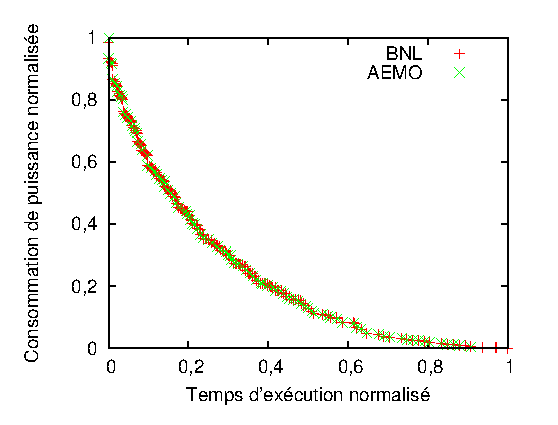
\includegraphics[scale=1.0]{chapitre6/chap6Fig/moea-bnl-norm.eps}
 \caption{Comparaison entre les solutions d'algorithme évolutionnaire et exhaustive.}
 \label{fig:moea-bnl-norm}
\end{figure}
Comme nous pouvons le voir sur la figure, les solutions résultantes de l'algorithme évolutionnaire et de l'algorithme BNL sont presque identiques avec une bonne répartition dans l'espace, ce qui signifie que l'AE peut trouver des solutions présentant un haut degré d'optimalité.
De plus, le temps d'exécution de l'AE est très faible comparé à celui de l'algorithme de recherche exhaustif, pour un $\mathcal{GGR}$ de 200 requêtes, le premier prend 7 secondes tandis que le second prend 4 jours sans avoir terminé son exécution.
Le \ref{tab:moea-exec-time} montre le temps d'exécution que l'AE a dépensé pour la génération des points de frontière de Pareto lorsque le nombre de requêtes de requêtes et de vues augmente. L'algorithme BNL n'est pas pris en compte car il nécessite plusieurs jours pour terminer son exécution, même avec une implémentation multi-thread exécutée sur un serveur haut de gamme. Les résultats obtenus montrent que notre approche donne rapidement les meilleures solutions.

\begin{table}
\centering
\caption {Temps d'exécution de l'AE en fonction de la taille des charges de requêtes SSB.} \label{tab:moea-exec-time}
    \begin{tabular}{ccc}
    \toprule
    \textbf{Nombre de requêtes} & \textbf{Vues candidates} & \textbf{Temps d'exécution (sec)} \\
	\midrule
	15 & $2^{23}$ & 2 \\
    30 & $2^{34}$ & 2 \\
    100 & $2^{70}$ & 4 \\
    200 & $2^{88}$ & 7 \\
    \bottomrule
    \end{tabular}
\end{table}

\subsubsection{Impact des coûts d'E/S et CPU}\label{subsubsec:ImpactIOCPUCosts}
Le but de cette expérimentation est d'étudier les profils de performance et d'énergie des configurations de vues matérialisées. Cela nous aide à mieux comprendre l'impact des coûts d'E/S et CPU de vues et leurs relations avec la performance et la consommation d'énergie. Sur la base de ces connaissances, nous pouvons concevoir les bases de données en tenant compte des stratégies d'économies et d'efficacité énergétique.
Nous avons utilisé notre charge de 30 requêtes SSB pour générer le $\mathcal{GGR}$ correspondant, puis en utilisant l'algorithme évolutionnaire, en obtient les configurations de vues matérialisée dominantes. Ensuite, nous prenons les configurations VM-Temps, VM-Puissance, VM-Compromis et nous calculons leurs temps d'exécution, consommation d'énergie, le coût total d'E/S, et le coût total de CPU. Les résultats sont présentés dans la \ref{fig:power-time-io-cpu-histo}.
\begin{figure}
  \centering
  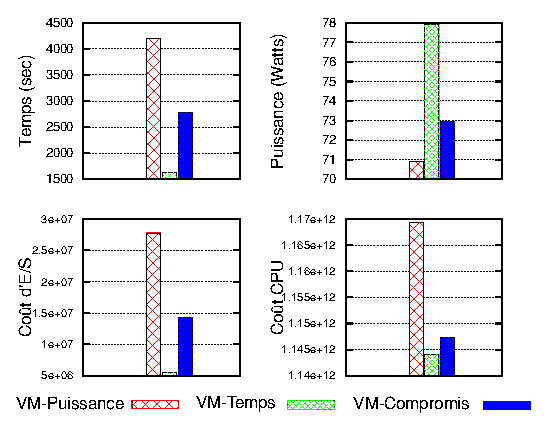
\includegraphics[width=0.6\textwidth]{chapitre6/chap6Fig/power-time-io-cpu-histo.eps}
  \caption{Les caractéristiques des vues matérialisées et leurs impacts sur la performance et la consommation d'énergie.}\label{fig:power-time-io-cpu-histo}
\end{figure}
À partir de cette dernière, nous remarquons que : (1) la configuration VM-Temps est caractérisée par un nombre minimal des coûts d'E/S et de CPU, qui conduisent à un temps d'exécution court, mais une forte consommation d'énergie, (2) VM-Puissance a des coûts d'E/S et de CPU élevés, conduisant à une faible consommation d'énergie avec un temps d'exécution long, (3) dans la configuration VM-Compromis, les coûts et le temps/puissance sont dans des valeurs de compromis.
L'observation immédiate est que le temps d'exécution et le coût d'E/S sont presque identiques dans toutes les configurations, ce qui est déjà connu dans l'optimisation des bases de données traditionnelles en raison du temps de traitement CPU rapide par rapport aux périphériques d'E/S. La seconde observation est que ni le coût d'E/S, ni le coût de CPU contribuent directement à la consommation d'énergie.
Notre interprétation est que pour certaines requêtes, l'opération de lecture de gros fichiers a besoin de tâches d'E/S supplémentaires. Lorsque les résultats intermédiaires ne peuvent pas tenus dans la mémoire, ils seront écrits sur le disque et lus plus tard. Cette surcharge est traduite par une augmentation du temps d'attente de CPU. En d'autres termes, l'optimiseur de requête passe plus de temps dans les opérations de lecture/écriture au lieu de traiter les données. Ainsi, les requêtes dominées par des coûts d'E/S ont une moindre consommation de puissance électrique. D'un autre côté, quand la taille des fichiers est petite, l'opération de lecture de données se termine rapidement et en son temps restant, la requête est dominée par le processeur. Cela peut se traduire par une consommation de puissance électrique élevée. Ainsi, pour produire des vues matérialisées avec un compromis entre la performance et la puissance électrique, nous recommandons de choisir des vues avec des coûts moyens d'E/S et de CPU.

\subsubsection{Impact d'espace de stockage}\label{subsubsec:ImpactStorageSpace}
Dans cette série d'expérimentations, nous considérons la contrainte de l'espace de stockage. Soit $S$ l'espace de stockage nécessaire pour sauvegarder tous les vues candidates; $S$ se varie de 5\% à 100\%; la charge de requêtes est la même que celle utilisée dans les expérimentations précédentes (30 requêtes OLAP basées sur le benchmark SSB). Nous calculons la qualité des solutions ($Q_s$), qui est exprimée par le ratio entre le coût de chaque solution et les meilleurs coûts des solutions que notre algorithme peut obtenir lorsque les contraintes sont ignorées. L'optimalité de Pareto (cf. \ref{sec:Multi-objective} [page \pageref{sec:Multi-objective}]) implique que, dans certains cas, $Q_s$ est supérieur à 1. Cependant, plus la valeur du $Q_s$ est proche à 1, plus la qualité de la solution est meilleure. Pour chaque type de configuration, nous calculons la variation des qualités des solutions pour la charge de requêtes en fonction de temps d'exécution et de la consommation d'énergie, par rapport à l'espace de stockage alloué pour les vues matérialisées. Les résultats sont tracés dans la \ref{fig:mv-size}.
Nous notons que la qualité des solutions s'améliore quand $S$ est plus relaxé. Ceci est dû au fait qu'il y aura plus d'espace disque pour stocker les vues matérialisées.
À partir de la même figure, on remarque que l'algorithme évolutionnaire trouve la meilleure solution pour VM-Temps rapidement, exactement à partir du point $S = 30\%$ (c-à-d $Q_s = 1$), ce n'est pas le cas pour la VM-Puissance, où la meilleure solution est obtenue quand $S$ est à 45\%. En conséquence, la configuration VM-Compromis est devenue stable jusqu'à $S = 70\%$. Ceci est dû à la diversité des solutions apportées par l'algorithme évolutionnaire; un bon compromis peut être vu quand $S$ prend une valeur comprise entre 70\% et 100\% de l'espace total.
La \ref{fig:mv-size} montre également que les valeurs de performance et de puissance évoluent en sens inverses (lorsque la puissance est élevée, le temps est court et vice versa), cela correspond au principe des frontières de Pareto discutés précédemment.
\begin{figure}
  \centering
  \subfloat[L'impact du contrainte d'espace de stockage.\label{fig:mv-size}]{
    \centering
    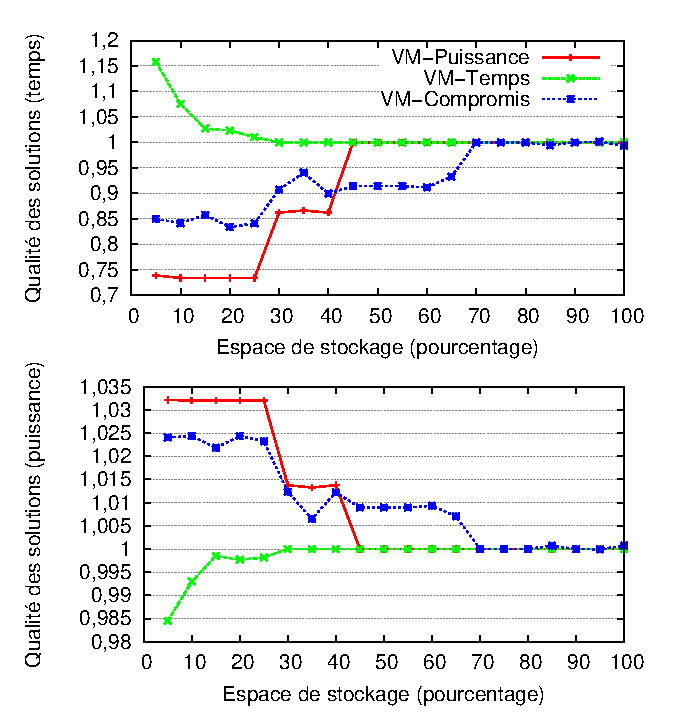
\includegraphics[width=0.45\textwidth]{chapitre6/chap6Fig/mv-size.eps}
  }
  \quad
  \subfloat[L'impact du contrainte du coût de maintenance.\label{fig:mv-maint}]{
    \centering
    \includegraphics[width=0.45\textwidth]{chapitre6/chap6Fig/mv-maint.eps}
  }
  \caption{Qualité des solutions en terme de performance et de consommation d'énergie avec la contrainte des ressources.}\label{fig:mv-const-relaxed}
\end{figure}

\subsubsection{Impact du coût de maintenance}\label{subsubsec:ImpactMaintenance}
Le but de cette expérimentation est de sélectionner un ensemble de vues, tout en respectant la contrainte des coûts de maintenance. Cette contrainte est évaluée comme suit. Soit $T$ le temps de maintenance de vue totale, lorsque le résultat de chaque nœud candidat de la charge de requêtes est matérialisé; $T$ se varie entre 5\% et 100\%. Dans la \ref{fig:mv-maint}, la qualité des solutions trouvées par notre approche en termes de temps d'exécution et de consommation d'énergie est illustrée. De même que pour la contrainte d'espace, la qualité des solutions s'améliore quand $T$ devient plus relaxé, car ça nécessite plus de temps pour maintenir les vues matérialisées.
Comme nous pouvons le voir sur la même figure, la meilleure solution pour VM-Puissance est trouvée quand $T$ est à 10\%, tandis que les autres configurations ont convergé vers la meilleure solution quand $T$ atteint 50\%. Cela est dû à la haute intensité énergétique de la tâche de maintenance, car elle implique de nombreuses opérations de comparaison pour calculer le changement dans la relation de base, ce qui impliquent plus de tâches de CPU supplémentaires et une consommation d'énergie élevée. La meilleure solution de compromis est trouvée rapidement par rapport au cas de la contrainte de l'espace, bien que les deux contraintes semblent similaires, elles se distinguent par une différence significative. L'espace occupé par un ensemble de vues augmente toujours quand une nouvelle vue est insérée, alors ce n'est pas le cas pour le coût de maintenance; il est possible de diminuer le temps de mise à jour d'un ensemble de vues après l'ajout d'une nouvelle vue \cite{Mami12}. Ceci est clairement reflété par la \ref{fig:mv-maint}, quand $T$ est entre 5\% et 25\% de l'intervalle de temps total, les solutions sont plus efficaces en terme de performances. D'autre part, quand $T$ est entre 25\% et 50\% les solutions sont plus efficaces en terme d'énergie. Quand $T$ dépasse 50\%, l'intervalle de temps devient suffisant pour obtenir la meilleure solution de compromis.

\subsubsection{Impact d'espace de stockage et du coût de maintenance}\label{subsubsec:ImpactMaintenanceStorage}

\begin{figure}
  \centering
  \subfloat[L'impact du contrainte d'espace de stockage ($T = 20\%$).\label{fig:mv-size-maint}]{
    \centering
    \includegraphics[width=0.45\textwidth]{chapitre6/chap6Fig/mv-size-maint.eps}
  }
  \quad
  \subfloat[L'impact du contrainte du coût de maintenance ($S = 40\%$).\label{fig:mv-maint-size}]{
    \centering
    \includegraphics[width=0.45\textwidth]{chapitre6/chap6Fig/mv-maint-size.eps}
  }
  \caption{Qualité des solutions en terme de performance et de consommation d'énergie avec différentes combinaisons de contraintes.}\label{fig:mv-const-combined}
\end{figure}

Afin d'examiner l'impact des contraintes d'espace de stockage et du coût de maintenance sur la qualité des solutions, nous procédons à cette série d'expérimentations. Dans le premier cas, nous avons fixé l'intervalle de temps $T$ à 20\% et nous avons varié les valeurs de la contrainte de l'espace $S$ de 5\% à 100\%. Dans la \ref{fig:mv-size-maint}, nous illustrons la qualité des solutions fournies par l'AE pour les différentes valeurs de $S$. Nous observons que seule la configuration VM-Puissance converge vers la meilleure solution, tandis que la configuration VM-Temps ne converge pas dans les deux objectifs à savoir le temps d'exécution et la consommation d'énergie (c'est à dire, $Q_s \approx 1,3$, $Q_s \approx 0,97$ respectivement). Cela conduit au fait que dans cette situation, les valeurs restrictives de la contrainte de maintenance produisent des solutions qui sont efficaces en terme d'énergie, mais avec un temps d'exécution important. Par conséquent, la solution de compromis n'est pas atteinte, même lorsque le $S$ est complètement relaxé, parce que la contrainte de coût de maintenance devient le facteur dominant.

Dans le deuxième cas, nous avons fixé l'espace de stockage $S$ à 40\% et nous avons varié les valeurs de la contrainte de maintenance $T$ de 5\% à 100\%. La \ref{fig:mv-maint-size} montre les résultats de la qualité des solutions lorsque $T$ est varié. Encore une fois, une seule configuration qui est VM-Temps converge vers la meilleure solution, les deux autres ne parviennent pas à converger même quand $T$ est totalement relaxé (c'est à dire, $Q_s \approx 0,9$ pour le temps et $Q_s \approx 1.015$ pour l'énergie), ceci est dû au fait que la contrainte d'espace est un facteur dominant dans cette situation. En outre, les résultats indiquent que les valeurs restrictives des solutions favorisent d'espace de stockage avec un faible temps d'exécution, mais la consommation d'énergie est importante. De même à la \ref{fig:mv-maint}, les solutions de compromis changent de façon significative avec la variation du temps de maintenance, cela étaie nos constatations dans l'expérimentation de la \ref{subsubsec:ImpactMaintenance}, la meilleure valeur ne peut être vu qu'à $T = 25\%$.

Les résultats présentés ci-dessus montrent clairement l'impact des contraintes d'espace de stockage et de maintenance sur la performance/énergie dans le processus de conception physique de la base de données. Par conséquent, le DBA doit définir les paramètres des contraintes de stockage et de maintenance attentivement pour obtenir un bon compromis entre les deux objectifs ou donner la priorité à des solutions orientées performance ou énergie.

\subsubsection{Impact des fréquences de mises à jour des vues}\label{subsubsec:ImpactViewsUpdateFrequency}
\begin{figure}
 \centering
 \includegraphics[scale=0.7]{chapitre6/chap6Fig/mv-update-freq.eps}
 \caption{Qualité des solutions en terme de performances et de consommation d'énergie avec différentes fréquences de mises à jour ($S = 40\%$).}
 \label{fig:mv-update-freq}
\end{figure}

Dans les expérimentations précédentes, nous avons supposé que la fréquence de mises à jour des vues $f_v$ était uniforme. Dans cet ensemble d'expérimentations, nous varions les valeurs de $f_v$ de 0,01 à 25 et nous fixons l'espace de stockage $S$ à 40 \% afin d'étudier l'impact de la fréquence de mises à jour des vues sur la qualité des solutions. La \ref{fig:mv-update-freq} illustre la relation entre la qualité des solutions et la fréquence de mises à jour des vues en terme de performance et de puissance. À partir de cette figure, nous observons que des valeurs faibles de $f_v$ (entre 0,01 et 1) produisent des solutions de bonne qualité pour toutes les configurations de vues matérialisées en terme de performance et de puissance. Cependant, lorsque $f_v$ est élevé (entre 1 et 25), la qualité des solutions des configurations VM-Temps et VM-Compromis est devenue mauvaise, seule la configuration VM-Puissance donne toujours les solutions les plus proches aux meilleurs ensembles. Rappelons que la fréquence de mises à jour a un impact sur le coût de maintenance (c'est-à-dire l'\ref{eq:maint-cost-model}) et le coût total de la charge. Par conséquent, des valeurs élevées de $f_v$ augmentent les coûts des requêtes et conduisent à la réduction des ensembles de solutions satisfaisant les contraintes. De ce fait, on produit des solutions de mauvaise qualité, notamment pour la configuration VM-Temps. A partir des résultats ci-dessus, nous concluons que des valeurs très élevées de fréquence de mises à jour ont un impact majeur sur la qualité des solutions de vues matérialisées. Par conséquent, ce cas devrait être pris en considération par le DBA.

\subsubsection{Évaluation avec le scénario d'énergie comme contrainte}\label{subsubsec:ImpactPower}
Supposons un scénario où un fournisseur de services tel qu'un centre de calcul ou un opérateur de Cloud Computing veut optimiser une charge de requêtes, en sélectionnant un ensemble de vues matérialisées qui réduisent la consommation d'énergie, tout en conservant un objectif de performance prédéfini. Cette situation est commune dans un environnement de Cloud où la tendance actuelle est << base de données en tant que de service >> (\gls{DBaaS}). Dans telles situations, l'objectif est de répondre à des contrats de service (\gls{SLA}) et d'optimiser l'utilisation des ressources telles que la consommation d'énergie, afin de maximiser les marges bénéficiaires. Nous proposons d'utiliser notre méthodologie pour aider les opérateurs à identifier la valeur minimale d'énergie qui assure une performance conforme au SLA établi. Dans ce scénario, la consommation d'énergie devient une contrainte à satisfaire. Le nouveau problème $\mathcal{PSV}$ est formalisé comme suit : pour (i) un schéma de base de données $BD$; (ii) une charge de requêtes $\mathcal{W}$; (iii) une contrainte de consommation d'énergie $P$; (iv) un $\mathcal{BNF}$ représentant le coût de traitement des requêtes. Le $\mathcal{PSV}$ consiste à sélectionner un ensemble de vues matérialisées $VM = \{V_1, V_2, \cdots, V_m\}$ réduisant le coût de traitement des requêtes et garantissant que la consommation d'énergie ne dépasse pas le seuil $P$.

Soit $P$ la puissance électrique de la charge de requêtes lorsque tous les vues sont matérialisées moins la puissance de l'exécution de la charge requêtes sans matérialisation; $P$ se varie de 5\% à 100\%. Le SLA est défini comme étant le temps d'exécution de la meilleure solution de compromis que notre AE peut trouver. Pour chaque valeur de $P$, on définit la violation d'une solution du contrat SLA comme le rapport de la durée d'exécution de cette solution sur le temps d'exécution de la meilleure solution. Notez que nous relaxons les deux autres contraintes. Les résultats de l'expérience sont récapitulés dans le \ref{tab:power-const}. De la table, nous pouvons voir qu'en utilisant notre technique, la violation du SLA descend à 0 lorsque $P = 45\%$. Ainsi, le réglage de la puissance électrique à cette valeur garantit le respect de SLA et produit un bénéfice de 20,8\% d'économie d'énergie.

Les résultats confirment l'efficacité de notre méthode pour aider les opérateurs de service à trouver les bons paramètres pour un meilleur compromis entre la performance et l'efficacité énergétique. En outre, il peut être utilisé comme un provisionnement dynamique des ressources par les fournisseurs de services pour allouer dynamiquement un nombre minimal de ressources nécessaires pour satisfaire une qualité de service spécifique. Par la suite, nous allons évaluer les économies d'énergie que l'approche proposée peut atteindre.

\begin{table}
\caption {Impact de la contrainte de puissance électrique.} \label{tab:power-const}
\centering
    \begin{tabular}{ccc}
    \toprule
    \multicolumn{1}{c}{\begin{tabular}[c]{@{}c@{}}\textbf{Limite}\\ \textbf{de puissance (\%)}\end{tabular}} & \multicolumn{1}{c}{\begin{tabular}[c]{@{}c@{}}\textbf{Violation}\\ \textbf{de SLA (\%)}\end{tabular}} & \multicolumn{1}{c}{\begin{tabular}[c]{@{}c@{}}\textbf{Économie}\\ \textbf{d'énergie (\%)}\end{tabular}} \\
	\midrule
	5	& 46,59 &	28,95 \\
	10	& 32,79 &	27,32 \\
	15	& 27,45 &	26,58 \\
	20	& 24,91 &	26,18 \\
	25	& 16,73 &	24,75 \\
	30	& 11,73 &	23,77 \\
	35	& 11,73 &	23,77 \\
	40	& 11,73 &	23,77 \\
	45	& 0 & 20,81 \\
    \bottomrule
    \end{tabular}
\end{table}

\subsubsection{Économie d'énergie et de puissance électrique}\label{subsubsec:PowerEnergySaving}
Le but de cette série d'expérimentations est d'étudier les avantages de notre approche en termes d'efficacité énergétique dans le scénario << énergie comme un $\mathcal{BNF}$ >> . Nous allons étudier deux cas en ce qui concerne la puissance électrique et l'économie d'énergie : (i) par requête et (ii) par la charge de requêtes. Dans le premier cas, en utilisant notre simulateur, nous exécutons tous les 30 requêtes OLAP du benchmark SSB avec une taille de base de données de 100 Go utilisant les configurations de vues matérialisées VM-Temps et VM-Puissance. Nous collectons les coûts de performances et de consommation d'énergie pour chaque configuration. Nous calculons la puissance/économie d'énergie et de la dégradation des performances de VM-Puissance par rapport à VM-Temps en utilisant les formules suivantes (à savoir, le cas d'économie d'énergie) pour la requête $Q_i$ :
\begin{equation}\label{eq:power-saving}
 EconomieEnergie_i = \frac{Energie_i - Energie_{VM-Temps}}{Energie_{VM-Temps}} \times 100
\end{equation}

\begin{figure}
  \centering
  \includegraphics[width=0.6\textwidth]{chapitre6/chap6Fig/ssb-mv-conf.eps}
  \caption{Impact des configurations de vues matérialisées sur les performances et la consommation d'énergie des requêtes SSB.}\label{fig:ssb-mv-conf}
\end{figure}

Dans la \ref{fig:ssb-mv-conf}, les résultats d'économie d'énergie et la dégradation de performance en pourcentage sont affichés. Comme nous pouvons le remarquer, 21 des 30 requêtes ont le potentiel d'économie d'énergie dans la configuration VM-Puissance. En principe, le bénéfice de la conservation de l'énergie pour ces requêtes à un impact négatif sur le temps de traitement comme indiqué dans la même figure. Cependant, comme nous allons le démontrer, le choix de la configuration de compromis (VM-Compromis) peut conduire à de bonnes valeurs d'économie d'énergie avec moins de dégradation des performances. Ces requêtes sont caractérisées par un nombre important d'opérateurs SQL, diverses opérations d'E/S et de CPU, et partagent beaucoup d'opérateurs SQL communs. Il en résulte un riche $\mathcal{GGR} $ et offre au algorithme évolutionnaire une variété de choix de configurations de vues. Par conséquent, nous pouvons avoir des requêtes offrant une bonne économie d'énergie à partir de ces vues, car les composants les plus intensifs en puissance électrique seront matérialisés. D'autre part, le reste de requêtes qui ne présentent pas de possibilités d'économie d'énergie, sont des requêtes avec un petit nombre d'opérateurs SQL et un ensemble limité de composants partagés. Cela conduit l'algorithme évolutionnaire à choisir les mêmes vues dans les deux configurations VM-Temps et VM-Puissance. Nous concluons qu'il existe des possibilités de conservation de l'énergie au \textit{niveau de requête} en utilisant une technique d'optimisation orientée-énergétique dans la conception physique.

Dans le second cas, nous nous concentrons notre attention sur le \textit{niveau de la charge de requêtes}. Plus précisément, nous créons trois charges de requêtes à partie de SSB : (1) WL30 contient 30 requêtes, (2) WL100 contient 100 requêtes, et (3) WL200 contient 200 requêtes. Pour chaque jeu de requête, nous générons leurs $\mathcal{GGR}$ en utilisant notre simulateur pour obtenir les coûts de performances, de puissance et la consommation d'énergie pour les trois configurations de vues matérialisées (VM-Temps, VM-Puissance, VM-Compromis du \ref{tab:mv-charact}) avec la relaxation des contraintes. En outre, nous calculons les coûts initiaux de la charge de requêtes sans optimisation afin de les exploiter dans la partie de comparaison. Nous exécutons les expérimentations sur deux tailles de bases de données différentes : 10 Go et 100 Go. Nous calculons l'économie de la puissance/d'énergie et de la dégradation des performances de VM-Puissance et VM-Compromis par rapport à la configuration VM-Temps, en utilisant l'\ref{eq:power-saving}.

\begin{table}
%\small
\footnotesize
%\scriptsize
\centering
\caption{Économies de puissance/énergie et dégradation de performance dans différentes configurations des vues matérialisées.}\label{tab:power-energy-saving}
\begin{tabular}{cllcccccc}
\toprule
\begin{tabular}[c]{@{}c@{}}\textbf{Taille}\\ \textbf{BD}\end{tabular} & \multicolumn{1}{c}{\begin{tabular}[c]{@{}c@{}}\textbf{Charge}\\ \textbf{Req}\end{tabular}} & \multicolumn{1}{c}{\begin{tabular}[c]{@{}c@{}}\textbf{Conf}\\ \textbf{MV}\end{tabular}} & \multicolumn{1}{c}{\begin{tabular}[c]{@{}c@{}}\textbf{Temps}\\ \textbf{(min)}\end{tabular}} & \multicolumn{1}{c}{\begin{tabular}[c]{@{}c@{}}\textbf{Puissance}\\ \textbf{(W)}\end{tabular}} & \multicolumn{1}{c}{\begin{tabular}[c]{@{}c@{}}\textbf{Énergie}\\ \textbf{(kJ)}\end{tabular}} & \multicolumn{1}{c}{\begin{tabular}[c]{@{}c@{}}\textbf{Économie}\\ \textbf{Puissance (\%)}\end{tabular}} & \multicolumn{1}{c}{\begin{tabular}[c]{@{}c@{}}\textbf{Économie}\\ \textbf{Énergie (\%)}\end{tabular}} & \multicolumn{1}{c}{\begin{tabular}[c]{@{}c@{}}\textbf{Deg}\\ \textbf{Perf (\%)}\end{tabular}} \\
\midrule
\multirow{12}{*}{10 Go}    &     \multirow{4}{*}{WL30}     & Origine & 45,83 & 15,29 & 42,04 & - & - &    -      \\
 &  &     VM-Temps         & 7,92 & 20,91 & 9,93 &  -  &  -  &    -      \\
    &       &     VM-Puissance        & 29,58 & 15 & 26,62 &  28,26  &  168,02  &    273,62      \\
    &       &     VM-Compromis    & 13,69 & 16,75 & 13,75 &  19,9  &  38,48  &    72,89      \\
    \noalign{\smallskip}
    %\midrule
    \cline{2-9}
    \noalign{\smallskip}
    %\midrule
    &     \multirow{4}{*}{WL100}   & Origine & 174,42 & 18,95 & 198,33 & - & - &    -      \\
 &  &     VM-Temps         & 87,23 & 23,82 & 124,66 &  -  &  -  &    -      \\
    &       &     VM-Puissance        & 222,15 & 16,87 & 224,85 &  29,17  &  80,38  &    154,66      \\
    &       &     VM-Compromis    & 138,69 & 19,41 & 161,53 &  18,49  &  29,59  &    58,99      \\
    \noalign{\smallskip}
    \cline{2-9}
    \noalign{\smallskip}
    &     \multirow{4}{*}{WL200}     & Origine & 350,86 & 19,03 & 400,55 & - & - &    -      \\
 &  &     VM-Temps         & 179,78 & 23,69 & 255,51 &  -  &  -  &    -      \\
    &       &     VM-Puissance        & 439,01 & 17,05 & 449,04 &  28,03  &  75,74  &    144,2      \\
    &       &     VM-Compromis    & 290,25 & 19,31 & 336,22 &  18,5  &  31,59  &    61,45      \\
    %\noalign{\smallskip}
    %\hline
    %\noalign{\smallskip}
    \midrule
\multirow{12}{*}{100 Go}     &     \multirow{4}{*}{WL30}     & Origine & 676,44 & 17,45 & 708,3 & - & - &    -      \\
 &  &     VM-Temps         & 190,81 & 25,61 & 293,19 &  -  &  -  &    -      \\
    &       &     VM-Puissance        & 1536,84 & 13,55 & 1249,14 &  47,1  &  326,04  &    705,43      \\
    &       &     VM-Compromis    & 241,17 & 22,79 & 329,8 &  11  &  12,49  &    26,39      \\
    \noalign{\smallskip}
    \cline{2-9}
    \noalign{\smallskip}
    &     \multirow{4}{*}{WL100}   & Origine & 2225,99 & 17,27 & 2306,09 & - & - &    -      \\
 &  &     VM-Temps         & 582,04 & 25,96 & 906,63 &  -  &  -  &    -      \\
    &       &     VM-Puissance        & 3963,11 & 13,67 & 3251,25 &  47,33  &  258,61  &    580,9      \\
    &       &     VM-Compromis    & 1487,87 & 16,8 & 1499,61 &  35,3  &  65,4  &    155,63      \\
    \noalign{\smallskip}
    \cline{2-9}
    \noalign{\smallskip}
    &     \multirow{4}{*}{WL200}   & Origine & 4459,49 & 17,4 & 4654,45 & - & - &    -      \\
 &  &     VM-Temps         & 1231,82 & 25,63 & 1894,56 &  -  &  -  &    -      \\
    &       &     VM-Puissance        & 8977,86 & 13,66 & 7358,2 &  46,71  &  288,39  &    628,83      \\
    &       &     VM-Compromis    & 3664,77 & 15,89 & 3493,13 &  38,03  &  84,38  &    197,51      \\
    \noalign{\smallskip}
    %\hline
    \bottomrule
\end{tabular}
\end{table}

Dans le \ref{tab:power-energy-saving} nous présentons les résultats des expérimentations (par exemple, l'économie d'énergie de la configuration de VM-Compromis avec une charge de requêtes 30WL et une taille de base de données de 10 Go est : $|\frac{16,75 - 20,91}{20,91}| \times 100\% = 19,9\%$). Nous pouvons voir clairement que les charges de requêtes consomment beaucoup moins d'énergie lorsque nous choisissons une configuration des vues matérialisées qui favorise des vues de faibles puissances électriques. Quand on compare les configurations puissance seule (VM-Puissance) avec performance seule (VM-Temps) des résultats, nous observons une marge importante des économies d'énergie, allant de 28\% à 47\%, le gain est remarquable quand nous allons de petite à grande taille de base de données et de charges de requêtes, cela est dû à la diversité des configurations de vues possibles en $\mathcal{GGR}$ d'une grande taille et leur impact sur la performance/puissance des systèmes. Ainsi, les expérimentations montrent des niveaux comparables d'économie d'énergie.
Comme on s'y attendait, les économies de la configuration VM-Compromis sont plus petites que celles obtenues par la configuration de puissance seule, mais elle réalise encore 11 à 38\% des valeurs d'économie.
D'autre part, la configuration de puissance prend plus de temps pour terminer l'exécution de toutes les requêtes, ce qui se traduit par une dégradation notable des performances. Ce résultat n'est pas étonnant puisque, si l'on gagne en puissance, nous perdons automatiquement en performance. Cependant, dans un scénario plus réaliste, un DBA est censé déployer la configuration VM-Compromis, dans laquelle la dégradation des performances est réellement acceptable si on la compare avec le cas d'optimisation (la colonne \textit{Origine} dans le \ref{tab:power-energy-saving}). En effet, par rapport au cas origine (aucune optimisation), nous gagnons toujours en puissance et économie d'énergie sans aucune dégradation de performance, en utilisant une configuration de compromis. Nous notons également que l'économie d'énergie totale de 12\% à 84\% dans le domaine de la recherche éco-énergétique, ce sont des taux intéressants et très prometteurs pour la conception des SGBDs plus efficaces en énergie.
En outre, pour la configuration de vues matérialisées en compromis, nous avons proposé un poids de 0,5 pour $\omega_1$ et $\omega_2$ pour les fonctions objectifs de performance et de puissance, mais dans les serveurs de base de données en monde réel, l'administrateur peut ajuster ces valeurs pour obtenir le compromis souhaité entre la conservation d'énergie et la dégradation de performance.

En résumé, les résultats obtenus prouvent que notre approche est valable. Avec notre configuration, nous obtenons des résultats encourageants pour économiser à la fois la puissance électrique et l'énergie. Si l'on considère un serveur de haute performance avec une puissance moyenne de 380 W, et en service continu, le serveur pourrait consommer pendant un an environ 3283 KWh d'énergie \cite{Barielle11}. Le coût de l'énergie total pour ce serveur unique serait de 328 dollars US par an (pour 10 centimes par kWh) en ignorant les coûts des systèmes d'infrastructure,  d'alimentation et de refroidissement \cite{Barielle11}. En utilisant les techniques proposées (12\% - 84\% d'économie d'énergie réalisée), en peut économiser 39 - 275 dollars US par serveur par an. Ce nombre pourrait augmenter pour les centres de calculs à grande échelle avec des milliers de serveurs.

\section{Conclusion}
Dans ce chapitre, nous avons proposé une initiative visant à intégrer l'énergie dans la phase physique du cycle de vie de la conception de base de données, en considérant le cas des vues matérialisées, une structure d'optimisation redondante.
%Avant de présenter nos démarches pour résoudre le problème la sélection des vues, nous avons donné une analyse approfondie de l'état le plus important des initiatives d'art couvrant à la fois le matériel et le logiciel.
Différents scénarios d'intégration de l'énergie dans le processus de sélection des vues matérialisées sont discutés. Dans cette étude, nous nous sommes concentrés sur deux scénarios : \textit{l'énergie comme un besoin non-fonctionnel} et \textit{l'énergie comme une contrainte}. Ces deux scénarios sont formalisés et résolus en utilisant des algorithmes évolutionnaires. Pour évaluer la qualité des solutions finales, nous avons développé des modèles de coûts mathématiques pour estimer les objectifs utilisés : consommation d'énergie et performances des requêtes. Des techniques d'apprentissage automatique ont été utilisées pour estimer les paramètres du modèle de coût dédié à la consommation d'énergie et le temps d'exécution. Ces modèles de coûts ont été utilisés pour évaluer notre proposition, et leurs résultats ont été comparés à ceux obtenus par la validation réelle.
En outre, nous avons souligné l'importance d'intégrer l'énergie dans la phase de conception physique pour avoir des bases de données éco-énergétiques. L'étude expérimentale confirme notre revendication, car l'approche proposée permet de réduire considérablement la consommation d'énergie globale de la charge de requêtes, en réalisant une \textit{économie de puissance active jusqu'à 38\%} et une \textit{économie d'énergie totale jusqu'à 84 \%}.
En outre, nous avons étudié un autre facteur très important dans les environnements de Cloud actuels, qui visent à réduire la consommation d'énergie tout en respectant un certain objectif de performance.
